\section{Communication}
Il a été décidé durant la phase de recherche que l'affichage se fera via un écran "volant" qui recevra les images via un réseau WiFi local
hébergé par le Raspberry Pi. Les étapes pour y arriver sont les suivantes:
\begin{enumerate}
    \item Flasher avec l'OS Raspberry (en utilisant Raspberry imager ou BalenaCloud).
    \item Être connecté à internet.
    \item Télécharger le package 'dnsmasq': \textbf{sudo apt-get install dnsmasq}.
    \item Atteindre le fichier suivant: \textbf{sudo nano /etc/wpa\char`_supplicant/wpa\char`_supplicant.conf}.
    \item Y ajouter le code du listing \ref{wpa}, sauver + quitter: ctrl+O, puis ctrl+X.
    \item Atteindre le fichier suivant: \textbf{sudo nano /etc/network/interfaces}.
    \item Y remplacer le code du listing \ref{interfaces}, sauver + quitter: ctrl+O, puis ctrl+X.
    \item Atteindre le fichier suivant: \textbf{sudo nano /etc/dnsmasq.conf}.
    \item Y remplacer le code du listing \ref{dnsmasq}, sauver + quitter: ctrl+O, puis ctrl+X.
    \item Redémarrer le Rpi4 avec: \textbf{sudo reboot}.
    \item Couper la connexion réseau avec: \textbf{sudo ifdown wlan0}.
    \item Accéder à la liste des réseaux avec: \textbf{sudo wpa\char`_cli -i wlan0 list\char`_networks}, puis saisir le réseau avec: \textbf{sudo wpa\char`_cli -i wlan0 select\char`_network 1} (exemple figure \ref{networks_list})
    \item Sauver la nouvelle configuration avec \textbf{sudo wpa\char`_cli -i wlan0 save\char`_config}.
    \item Relancer la connexion réseau avec: \textbf{sudo ifup \underline{wlan0=ap0}}.
\end{enumerate}
\begin{listing}[ht]
    \inputminted{makefile}{assets/figures/wpa_supplicant.make}
    \caption{Configuration wpa\char`_supplicant \label{wpa}}
\end{listing}

\begin{listing}[ht]
    \inputminted{makefile}{interfaces.make}
    \caption{Configuration de l'interface réseau \label{interfaces}}
\end{listing}

\begin{listing}[ht]
    \inputminted{makefile}{dnsmasq.make}
    \caption{Configuration dnsmasq \label{dnsmasq}}
\end{listing}

\begin{figure}[H]
    \centering
    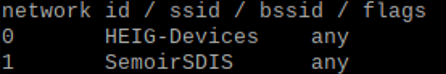
\includegraphics[width=13cm]{assets/figures/network_list.PNG}
    \caption{Liste de networks \label{networks_list}}
\end{figure}

Avec l'ajout de ces lignes, le Rpi4 émet un réseau local, pour que l'émission se fasse dès le démarrage de la carte,
il faut ouvrir le fichier suivant avec : \textbf{sudo nano /home/tb/.bashr} et y ajouter les lignes de codes des étapes \textbf{11 et 14}.

Il est possible de s'y connecter avec n'importe quel
type d'appareil. Le nom du réseau et le mot de passe sont paramétrables, actuellement, c'est:
\begin{itemize}
    \item Nom du réseau: \textbf{SemoirSDIS}
    \item Mot de passe: \textbf{123456789}
\end{itemize}\\
À noter qu'il est obligatoire de s'y connecter pour avoir le retour vidéo.

\begin{figure}[H]
    \centering
    
\includegraphics[width=3cm]{assets/figures/acces_wifi.PNG}
    \caption{QR code - Connexion WiFi local}
\end{figure}

\section{Affichage}
Il existe des codes sources disponibles en ligne permettant d'afficher le retour caméra basé sur le package Picamera2 \cite{picamera2}.
Je me suis inspiré de celui-ci pour mon affichage: \cite{code_camera}.

L'utilisation de \textbf{Picamera2} nécessite l'installation de dépendances:
\begin{itemize}
    \item \textbf{sudo apt-get install libatlas-base-dev}.
\end{itemize}
\textbf{Mettre screenshot du rendu sur natel/pc}

Mettre le code source en annexe.
\section{Accès}
L'accès au retour vidéo se fait via une page locale dont l'accès nécessite d'être connecté au WiFi émis par le Rpi4.
La page se trouve à l'adresse statique suivante:
\begin{itemize}
    \item  \url{192.168.0.1:8000/index.html}
\end{itemize}
Accès rapide:

\begin{figure}[H]
    \centering
    
\includegraphics[width=3cm]{assets/figures/acces_stream.PNG}
    \caption{QR code - Connexion Stream}
\end{figure}